\documentclass{beamer}
\usepackage{graphicx}
\usepackage{hyperref}

% Define Just Eat Takeaway color scheme
\usecolortheme[named=orange]{structure}
\setbeamertemplate{navigation symbols}{}
\setbeamertemplate{footline}[frame number]

\title{Data \& Analytics Case Study}
\author{Max van Rooijen (max@pl9.co)}
\date{\today}
\titlegraphic{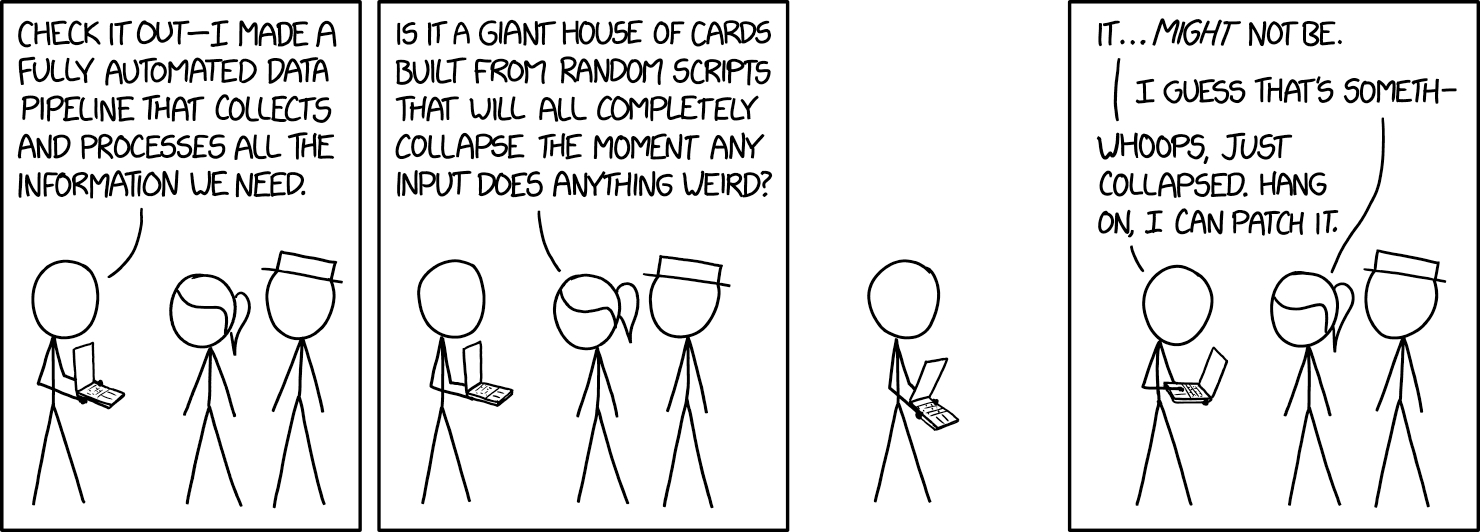
\includegraphics[width=0.9\textwidth]{../screenshots/data_pipeline_2x.png}}

\begin{document}

\frame{\titlepage}

\section{Why: The Need for Analytics in Comic Design}
\begin{frame}{Why Analytics in Comic Design?}
    \begin{columns}
        \column{0.5\textwidth}
        \begin{itemize}
            \item Understanding audience preferences and engagement
            \item Optimizing storytelling and visual elements
            \item Enhancing content personalization and recommendation
        \end{itemize}
        \column{0.5\textwidth}
        \centering
        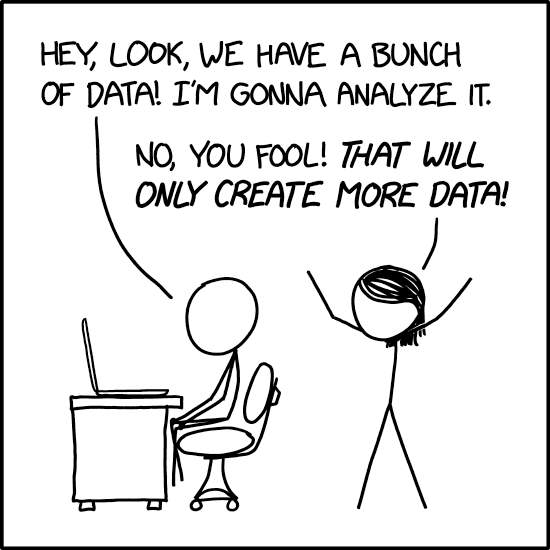
\includegraphics[width=0.9\textwidth]{../screenshots/data_trap_2x.png}
    \end{columns}
\end{frame}

\begin{frame}{Technical Solution: Batch Processing Pipeline}
    \begin{itemize}
        \item Fetching data from the XKCD API
        \item Using Apache Airflow to orchestrate workflows
        \item Staging data in a PostgreSQL Data Warehouse
        \item Transforming raw data using dbt (Data Build Tool)
        \item Running data quality checks to ensure integrity
    \end{itemize}
\end{frame}

\begin{frame}{Solution Overview}
    \centering
    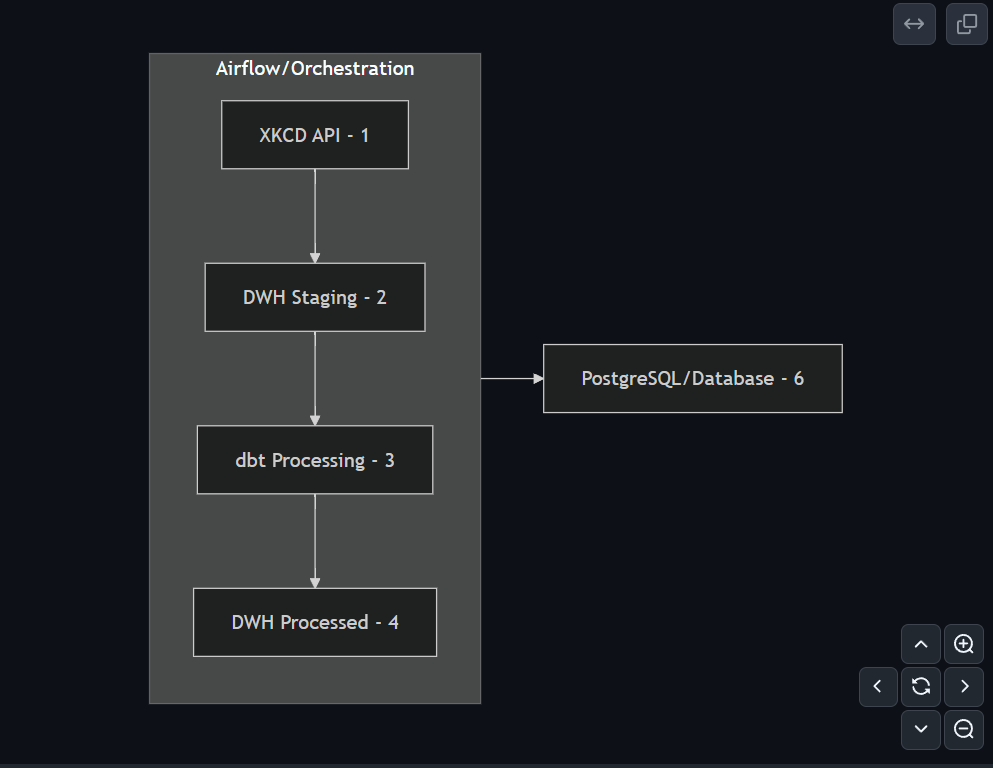
\includegraphics[width=0.8\textwidth]{../screenshots/solution_overview.png}
    \newline
    High-level overview of the architecture.
\end{frame}

\begin{frame}{Pipeline Architecture}
    \centering
    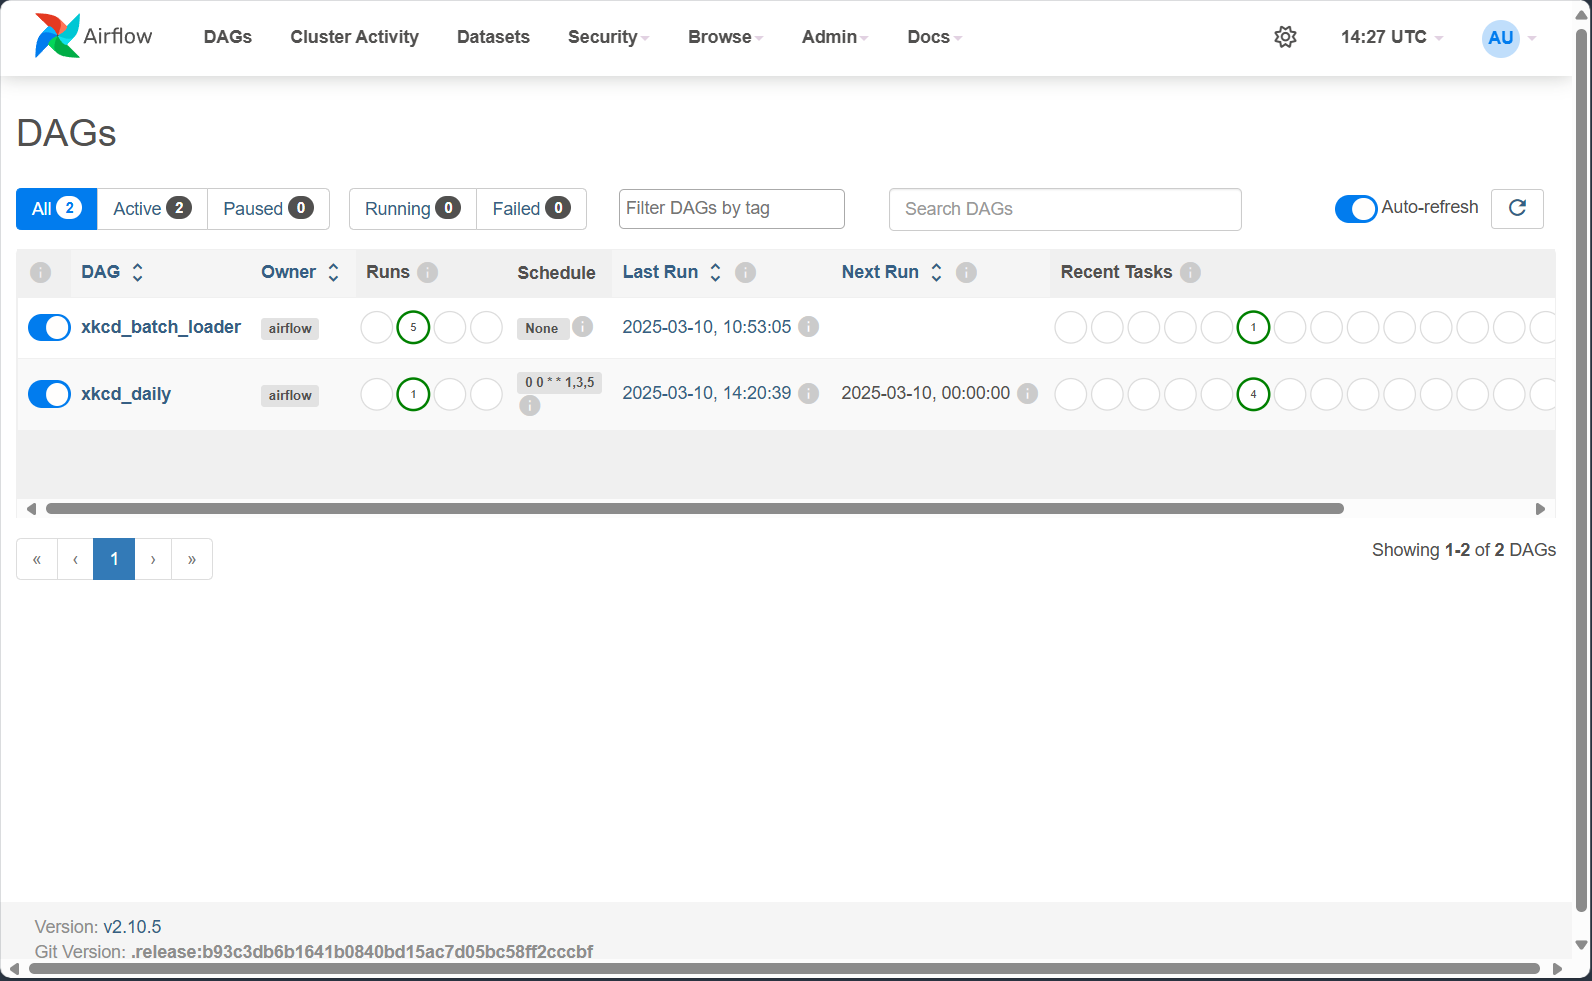
\includegraphics[width=0.8\textwidth]{../screenshots/airflow.png}
    \newline
    Overview of the DAGs in Airflow
\end{frame}

\begin{frame}{Pipeline Architecture}
    \centering
    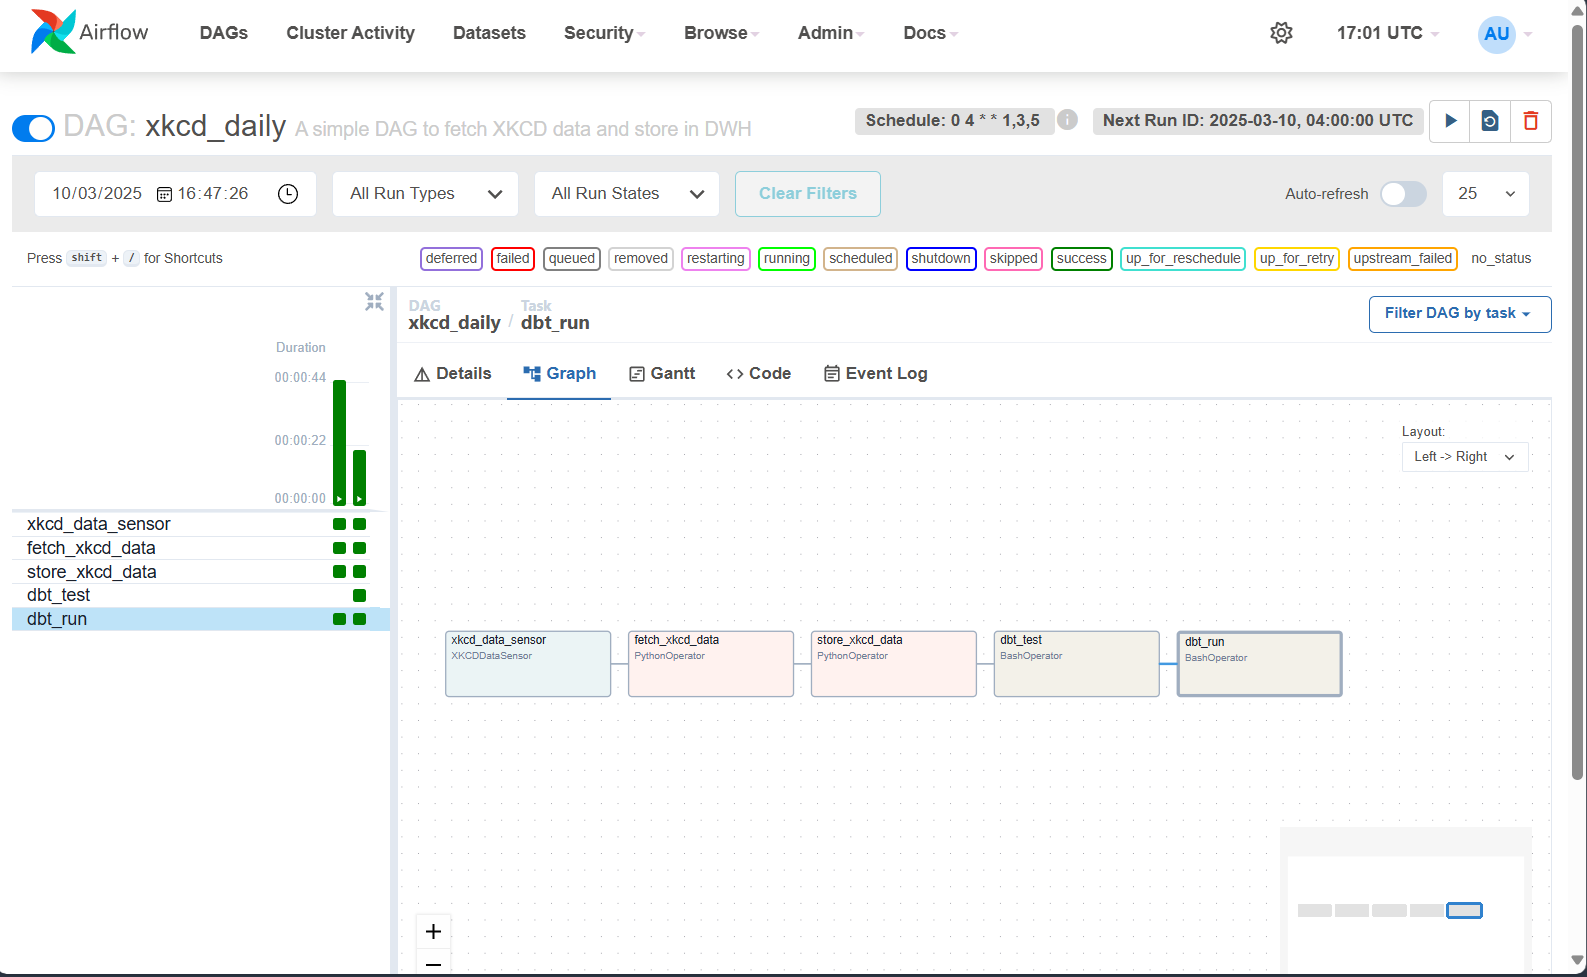
\includegraphics[width=0.8\textwidth]{../screenshots/airflow-dag.png}
    \newline
    Daily run DAG
\end{frame}

\begin{frame}{Data Model and Insights}
    \begin{itemize}
        \item Dimensional model for structured data storage
        \item Fact tables for costs, reviews, and views
        \item Aggregated insights for trend analysis
    \end{itemize}
    \centering
    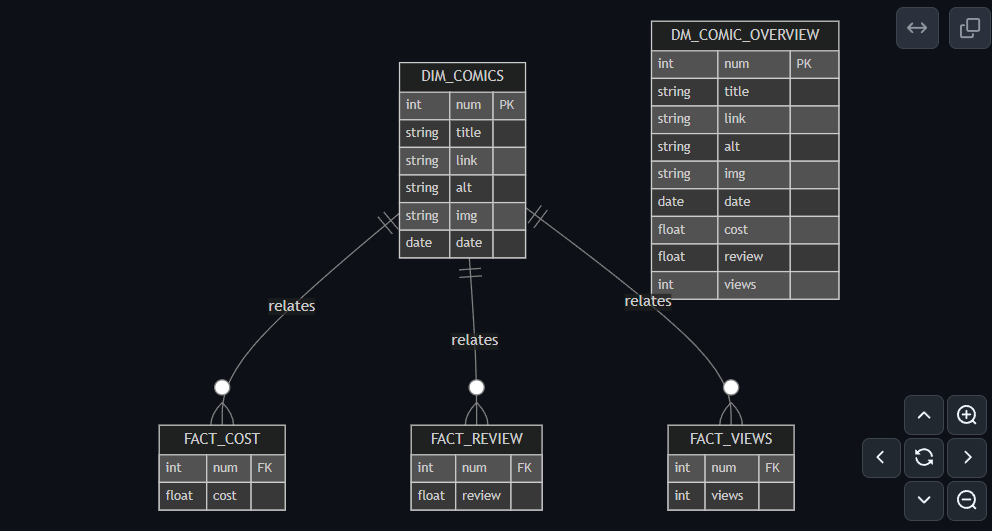
\includegraphics[width=0.8\textwidth]{../screenshots/er-diagram.png}
\end{frame}

\begin{frame}{Future Improvements}
    \begin{itemize}
        \item \textbf{Machine Learning Integration}: Use ML models for predictive insights, such as forecasting trends in comic engagement.
        \item \textbf{Enhanced Data Quality Checks}: Implement more comprehensive tests for duplicates, referential integrity, and outlier detection.
        \item \textbf{Unit Tests for DAGs}: Add unit tests to Airflow DAGs to ensure robust workflow execution.
        \item \textbf{More Elaborate Data Model}: Expand the data warehouse schema to include more detailed metadata and user behavior analytics.
        \item \textbf{Real-time Processing}: Extend the pipeline to support real-time analytics with streaming data solutions like Apache Kafka.
        \item \textbf{Scalability}: Optimize the data pipeline to handle larger volumes of data and improve performance.
        \item \textbf{Monitoring and Alerts}: Set up monitoring and alerting to notify the team of any issues or anomalies in the data pipeline.
        \item \textbf{Data Lineage}: Implement the dbt docs routine to automatically generate an interactive document in HTML and host it on a web server.
    \end{itemize}
\end{frame}

\section{Future: Business Cases and Opportunities}
\begin{frame}{Future Business Cases}
    \begin{itemize}
        \item \textbf{Optimizing Ad Placement}: Use insights from user engagement to strategically place advertisements in comics.
        \item \textbf{Personalized Content Recommendations}: Suggest comics based on reader preferences and past interactions.
        \item \textbf{Subscription \& Monetization Strategies}: Identify premium content opportunities based on high-engagement trends.
        \item \textbf{Predicting Viral Content}: Utilize data to forecast which comics are likely to go viral and maximize their exposure.
        \item \textbf{Expanding into New Media}: Apply the same analytical insights to animations, graphic novels, and interactive storytelling.
        \item \textbf{Improving Reader Retention}: Track engagement metrics to refine content strategy and keep readers coming back.
    \end{itemize}
\end{frame}

\end{document}
